
% This LaTeX was auto-generated from an M-file by MATLAB.
% To make changes, update the M-file and republish this document.

\documentclass{article}
\usepackage{graphicx}
\usepackage{color}
\usepackage{listings}
\usepackage[framed]{mcode}
\usepackage{fullpage}
\usepackage{amsmath}
\usepackage[utf8x]{inputenc}
\usepackage{import}
\usepackage{setspace}
\usepackage{hyperref}
\definecolor{lightgray}{gray}{0.5}
\setlength{\parindent}{0pt}

\begin{document}

    
    
%\section*{}

 \title{BE 521: Homework 4 \\{\normalsize HFOs}
\\{\normalsize Spring 2021}} \author{58 points} \date{Due: Tuesday,
2/23/2021 10:00pm} \maketitle \textbf{Objective:} HFO detection and
cross-validation 
 \begin{center} \author{NAME HERE \\
  \normalsize Collaborators: COLLABORATORS HERE \\}
\end{center}


\subsection*{HFO Dataset} High frequency oscillations (HFOs) are
quasi-periodic intracranial EEG transients with durations on the
order of tens of milliseconds and peak frequencies in the range of
80 to 500 Hz. There has been considerable interest among the
epilepsy research community in the potential of these signals as
biomarkers for epileptogenic networks.\\\\
In this homework exercise, you will explore a dataset of candidate
HFOs detected using the algorithm of Staba et al. (see article on
Canvas). The raw recordings from which this dataset arises come from
a human subject with mesial temporal lobe epilepsy and were
contributed by the laboratory of Dr. Greg Worrell at the Mayo Clinic
in Rochester, MN.\\\\
The dataset \verb|I521_A0004_D001| contains raw HFO clips that are
normalized to zero mean and unit standard deviation but are
otherwise unprocessed. The raw dataset contain two channels of data:
\verb|Test_raw_norm| and \verb|Train_raw_norm|, storing raw testing
and training sets of HFO clips respectively. The raw dataset also
contains two annotation layers: \verb|Testing windows| and
\verb|Training windows|, storing HFO clip start and stop times (in
microseconds) for each of the two channels above.
Annotations contain the classification by an ``expert'' reviewer
(i.e., a doctor) of each candidate HFO as either an HFO (2) or an
artifact (1). On ieeg.org and upon downloading the annotations,
You can view this in the "description" field. \\\\
After loading the dataset in to a \verb|session| variable as in
prior assignments you will want to familiarize yourself with the
\verb|IEEGAnnotationLayer| class. Use the provided "getAnnotations.m"
function to get all the annotations from a given dataset. The first
output will be an array of annotation objects, which you will see
also has multiple fields including a description field as well as start and stop times. Use
You can use the information outputted by getAnnotations to pull
each HFO clip.


\section{Simulating the Staba Detector (12 pts)} Candidate HFO clips
were detected with the Staba et al. algorithm and subsequently
validated by an expert as a true HFO or not. In this first section,
we will use the original iEEG clips containing HFOs and re-simulate
a portion of the Staba detection.
\begin{enumerate}
    \item How many samples exist for each class (HFO vs artifact) in
    the training set? (Show code to support your answer) (1 pt)

\begin{lstlisting}
cd('/Users/sppatankar/Developer/BE-521')
addpath(genpath('Homework_4'));
addpath(genpath('ieeg-matlab-1.14.49'))

session = IEEGSession('I521_A0004_D001', 'spatank', 'spa_ieeglogin.bin');

% training
hfo_num = 0;
artifact_num = 0;
[all_train_events, ~, ~] = ...
    getAnnotations(session.data, session.data.annLayer(1, 1).name);
train_cell_array = cell(1, length(all_train_events));
for i = 1:length(all_train_events)
    if all_train_events(1, i).description == '2'
        hfo_num = hfo_num + 1;
        train_cell_array{1, i}.description = all_train_events(1, i).description;
    end
    if all_train_events(1, i).description == '1'
        artifact_num = artifact_num + 1;
        train_cell_array{1, i}.description = all_train_events(1, i).description;
    end
    start_time = all_train_events(1, i).start; % microseconds
    end_time = all_train_events(1, i).stop; % microseconds
    duration = end_time - start_time;
    channel = 1;
    train_cell_array{1, i}.start = start_time;
    train_cell_array{1, i}.end = end_time;
    train_cell_array{1, i}.signal = ...
        session.data.getvalues(start_time, duration, channel);
end

% testing
[all_test_events, ~, ~] = ...
    getAnnotations(session.data, session.data.annLayer(1, 2).name);
test_cell_array = cell(1, length(all_test_events));
for i = 1:length(all_test_events)
    test_cell_array{1, i}.description = all_test_events(1, i).description;
    start_time = all_test_events(1, i).start; % microseconds
    end_time = all_test_events(1, i).stop; % microseconds
    duration = end_time - start_time;
    channel = 1;
    test_cell_array{1, i}.start = start_time;
    test_cell_array{1, i}.end = end_time;
    test_cell_array{1, i}.signal = ...
        session.data.getvalues(start_time, duration, channel);
end

% [ANSWER HERE]

% print to console
hfo_num
artifact_num
\end{lstlisting}

\color{lightgray} \begin{lstlisting}IEEGSETUP: Adding 'ieeg-matlab.jar' to dynamic classpath
IEEGSETUP: Found log4j on Java classpath.
URL: https://www.ieeg.org/services
Client user: spatank
Client password: ****

hfo_num =

   101


artifact_num =

    99

\end{lstlisting} \color{black}

    \item Using the training set, find the first occurrence of the
    first valid HFO and the first artifact.
        Using \verb|subplot| with 2 plots, plot the valid HFO's
        (left) and artifact's (right) waveforms. Since the units are
        normalized, there's no need for a y-axis, so remove it with
        the command \verb|set(gca,'YTick',[])|. (2 pts)

\begin{lstlisting}
first_hfo = 0;
hfo_idx = 0;
while first_hfo ~= 1
    hfo_idx = hfo_idx + 1;
    label = train_cell_array{1, hfo_idx}.description;
    if label == '2' % HFO found
        first_hfo = 1;
    end
end

first_artifact = 0;
artifact_idx = 0;
while first_artifact ~= 1
    artifact_idx = artifact_idx + 1;
    label = train_cell_array{1, artifact_idx}.description;
    if label == '1' % artifact found
        first_artifact = 1;
    end
end

sampling_rate = session.data.sampleRate;
dt = 1/sampling_rate;

hfo_start_time = train_cell_array{1, hfo_idx}.start/1e6; % s
hfo_end_time = train_cell_array{1, hfo_idx}.end/1e6; % s
hfo_time = hfo_start_time:dt:hfo_end_time;
hfo_signal = train_cell_array{1, hfo_idx}.signal;

artifact_start_time = train_cell_array{1, artifact_idx}.start/1e6; % s
artifact_end_time = train_cell_array{1, artifact_idx}.end/1e6; % s
artifact_time = artifact_start_time:dt:artifact_end_time;
artifact_signal = train_cell_array{1, artifact_idx}.signal;

% [ANSWER HERE]

figure;
subplot(1, 2, 1);
plot(hfo_time, hfo_signal, 'LineWidth', 1, 'Color', [0, 0, 0]);
xlim([hfo_time(1), hfo_time(end)])
xlabel('Time (s)', 'FontSize', 15);
title('HFO', 'FontSize', 15);
set(gca, 'YTick', []);

subplot(1, 2, 2);
plot(artifact_time, artifact_signal, 'LineWidth', 1, 'Color', [0, 0, 0]);
xlim([artifact_time(1), artifact_time(end)])
xlabel('Time (s)', 'FontSize', 15);
title('Artifact', 'FontSize', 15);
set(gca, 'YTick', []);
\end{lstlisting}


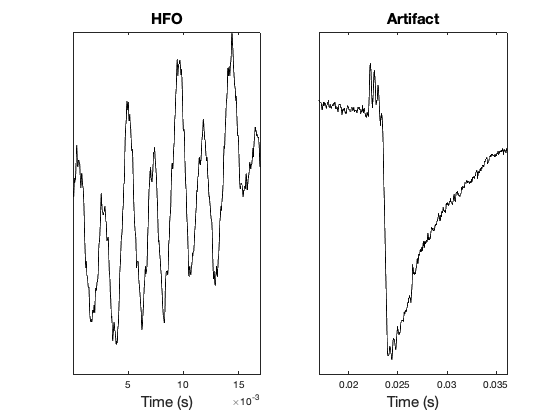
\includegraphics [width=5in]{spatank_hw4_01.png}

    \item Using the \texttt{fdatool} in MATLAB, build an FIR
    bandpass filter of the equiripple type of order 100.
        Use the Staba et al. (2002) article to guide your choice of
        passband and stopband frequency. Once set, go to
        \texttt{File} \verb|->| \texttt{Export}, and export
        ``Coefficients'' as a MAT-File. Attach a screenshot of your
        filter's magnitude response. (Note: We will be flexible with
        the choice of frequency parameters within reason.) (3 pts)

\begin{lstlisting}
% [ANSWER HERE]
\end{lstlisting}

    \item Using the forward-backward filter function
    (\texttt{filtfilt}) and the numerator coefficients saved above,
        filter the valid HFO and artifact clips obtained earlier.
        You will need to make a decision about the input argument
        \texttt{a} in the \texttt{filtfilt} function. Plot these two
        filtered clips overlayed on their original signal in a two
        plot \texttt{subplot} as before. Remember to remove the
        y-axis. (3 pts)

\begin{lstlisting}
% [ANSWER HERE]

load('Coefficients.mat');

hfo_signal_filt = filtfilt(Num, 1, hfo_signal);
artifact_signal_filt = filtfilt(Num, 1, artifact_signal);

figure;
subplot(1, 2, 1);
hold on
plot(hfo_time, hfo_signal, 'LineWidth', 1, 'Color', [0, 0, 0]);
plot(hfo_time, hfo_signal_filt, 'LineWidth', 1, 'Color', 'r');
hold off
xlim([hfo_time(1), hfo_time(end)])
ylim([min(hfo_signal), max(hfo_signal)])
legend('Raw', 'Filtered', 'Location', 'NorthEast');
xlabel('Time (s)', 'FontSize', 15);
title('HFO', 'FontSize', 15);
set(gca, 'YTick', []);

subplot(1, 2, 2);
hold on
plot(artifact_time, artifact_signal, 'LineWidth', 1, 'Color', [0, 0, 0]);
plot(artifact_time, artifact_signal_filt, 'LineWidth', 1, 'Color', 'r');
hold off
xlim([artifact_time(1), artifact_time(end)])
ylim([min(artifact_signal), max(artifact_signal)])
legend('Raw', 'Filtered', 'Location', 'NorthEast');
xlabel('Time (s)', 'FontSize', 15);
title('Artifact', 'FontSize', 15);
set(gca, 'YTick', []);
\end{lstlisting}


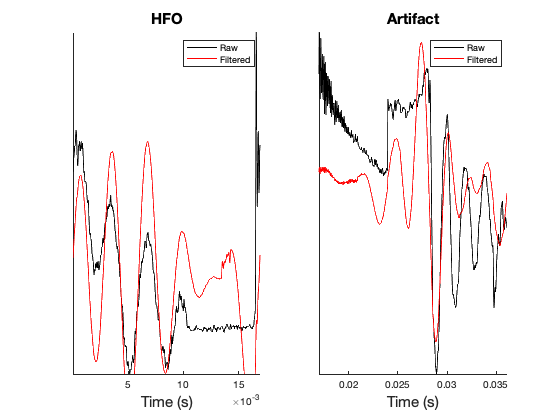
\includegraphics [width=5in]{spatank_hw4_02.png}

    \item Speculate how processing the data using Staba's method may
    have erroneously led to a false HFO detection (3 pts)

\begin{lstlisting}
% [ANSWER HERE]
\end{lstlisting}

\end{enumerate}
\section{Defining Features for HFOs (9 pts)} In this section we will
be defining a feature space for the iEEG containing HFOs and
artifacts. These features will describe certain attributes about the
waveforms upon which a variety of classification tools will be
applied to better segregate HFOs and artifacts
\begin{enumerate}
    \item Create two new matrices, \verb|trainFeats| and
    \verb|testFeats|, such that the number of rows correspond to
    observations (i.e. number of training and testing clips)
        and the number of columns is two. Extract the line-length and
        area features (seen previously in lecture and Homework 3) from
        the normalized raw signals (note: use the raw signal from
        ieeg.org, do not filter the signal). Store the line-length value
        in the first column and area value for each sample in the second
        column of your features matrices. Make a scatter plot of the
        training data in the 2-dimensional feature space, coloring the
        valid detections blue and the artifacts red. (Note: Since we only
        want one value for each feature of each clip, you will
        effectively treat the entire clip as the one and only
        ``window''.) (4 pts)

\begin{lstlisting}
% [ANSWER HERE]

LLFn = @(x) sum(abs(diff(x)));
areaFn = @(x) sum(abs(x));

trainFeats = zeros(length(train_cell_array), 2);
trainLabels = zeros(length(train_cell_array), 1);

for i = 1:length(train_cell_array)
    signal = train_cell_array{1, i}.signal;
    trainFeats(i, 1) = LLFn(signal);
    trainFeats(i, 2) = areaFn(signal);
    trainLabels(i, 1) = str2double(train_cell_array{1, i}.description);
end

figure;
gscatter(trainFeats(:, 1), trainFeats(:, 2), trainLabels, 'rb');
xlabel('Line Length (AU)', 'FontSize', 15);
ylabel('Area (AU)', 'FontSize', 15);
legend('Artifact', 'HFO', 'Location', 'SouthEast');
title('Feature Space', 'FontSize', 15);

testFeats = zeros(length(test_cell_array), 2);
testLabels = zeros(length(test_cell_array), 1);

for j = 1:length(test_cell_array)
    signal = test_cell_array{1, j}.signal;
    testFeats(j, 1) = LLFn(signal);
    testFeats(j, 2) = areaFn(signal);
    testLabels(j, 1) = str2double(test_cell_array{1, j}.description);
end
\end{lstlisting}


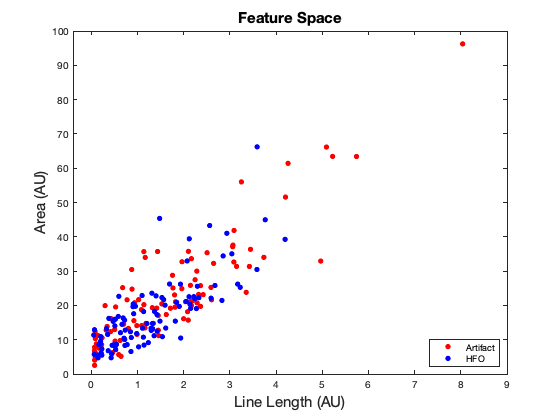
\includegraphics [width=5in]{spatank_hw4_03.png}

    \item Feature normalization is often important. One simple
    normalization method is to subtract each feature by its mean and
    then divide by its standard deviation
        (creating features with zero mean and unit variance). Using
        the means and standard deviations calculated in your
        \emph{training} set features, normalize both the training
        and testing sets. You should use these normalized features for
        the remainder of the assignment.
    \begin{enumerate} \item What is the statistical term for the
    normalized value, which you have just computed? (1 pt)

\begin{lstlisting}
trainFeatsNorm = (trainFeats - mean(trainFeats))./std(trainFeats);
testFeatsNorm = (testFeats - mean(trainFeats))./std(trainFeats);

% The normalized value is termed the z-score.
\end{lstlisting}

	\item Explain why such a feature normalization might be critical
	to the performance of a $k$-NN classifier. (2 pts)

\begin{lstlisting}
% $k$-NN uses a distance metric (often, the Euclidean distance) to
% iteratively cluster data points into groups. Large feature values can
% have a large contribution to the distance between points in feature
% space. By normalizing, every feature is assigned equal importance in
% determining distances.
\end{lstlisting}

\item Explain why (philosophically) you use the training feature means and
	standard deviations to normalize the testing set. (2 pts)

\begin{lstlisting}
% The test data is unseen during training time. As a result, any operations
% performed on this data should not be used when constructing the algorithm
% that will be tested on it. We also typically assume that descriptive statistics
% such as the mean and standard deviation hold for data points across the
% training and testing data sets, since all data comes from an underlying
% unseen distribution whose parameters we want to infer.
\end{lstlisting}

    \end{enumerate}
\end{enumerate}
\section{Comparing Classifiers (20 pts)} In this section, you will
explore how well a few standard classifiers perform on this dataset.
Note, the logistic regression, $k$-NN, and SVM classifiers are functions
built into some of Matlabs statistics packages. If you don't have
these (i.e., Matlab doesn't recognize the functions), and you are
experiencing any difficulty downloading the necessary packages, please
let us know.
\begin{enumerate}
 \item Using Matlab's logistic regression classifier function,
 (\texttt{mnrfit}), and its default parameters, train a model on the
 training set. Using Matlab's \texttt{mnrval} function, calculate
 the training error (as a percentage) on the data. For extracting
 labels from the matrix of class probabilities, you may find the
 command \texttt{[$\sim$,Ypred] = max(X,[],2)} useful\footnote{Note:
 some earlier versions of Matlab don't like the \texttt{$\sim$},
 which discards an argument, so just use something like
 \texttt{[trash,Ypred] = max(X,[],2)} instead.}, which gets the
 column-index of the maximum value in each row (i.e., the class with
 the highest predicted probability). (3 pts)

\begin{lstlisting}
% [ANSWER HERE]

Mdl_logistic = mnrfit(trainFeatsNorm, trainLabels);
[~, trainLabelsPred] = max(mnrval(Mdl_logistic, trainFeatsNorm), [], 2);

train_error_logistic = sum(trainLabels ~= trainLabelsPred)/length(trainLabels)
\end{lstlisting}

\color{lightgray} \begin{lstlisting}
train_error_logistic =

    0.4150

\end{lstlisting} \color{black}

 \item Using the model trained on the training data, predict the
 labels of the test samples and calculate the testing error. Is the
 testing error larger or smaller than the training error? Give one
 sentence explaining why this might be so. (2 pts)

\begin{lstlisting}
% [ANSWER HERE]

[~, testLabelsPred] = max(mnrval(Mdl_logistic, testFeatsNorm), [], 2);

test_error_logistic = sum(testLabels ~= testLabelsPred)/length(testLabels)
\end{lstlisting}

\color{lightgray} \begin{lstlisting}
test_error_logistic =

    0.3714

\end{lstlisting} \color{black}

 \item
  \begin{enumerate}
   \item Use Matlab's $k$-nearest neighbors function,
   \texttt{fitcknn}, and its default parameters ($k$ = 1, among
   other things), calculate the training and testing errors. (3 pts)

\begin{lstlisting}
% [ANSWER HERE]

Mdl_kNN = fitcknn(trainFeatsNorm, trainLabels);

trainLabelsPred = predict(Mdl_kNN, trainFeatsNorm);
train_error_knn = sum(trainLabels ~= trainLabelsPred)/length(trainLabels)

testLabelsPred = predict(Mdl_kNN, testFeatsNorm);
test_error_knn = sum(testLabels ~= testLabelsPred)/length(testLabels)
\end{lstlisting}

\color{lightgray} \begin{lstlisting}
train_error_knn =

     0


test_error_knn =

    0.4476

\end{lstlisting} \color{black}

   \item Why is the training error zero? (2 pts)

\begin{lstlisting}
% [ANSWER HERE]

% Matlab sets the number of neighbors used in the $k$-NN algorithm to 1 by
% default. As a result, each training point ends up being closest to itself
% and is accurately classified resulting in 0 training error.
\end{lstlisting}

  \end{enumerate}
 \item Now, train Matlab's implementation of a
 support vector machine (SVM), \texttt{fitcsvm}. Report the training and testing
 errors for an SVM model with a radial basis function (RBF) kernel function,
 while keeping other parameters at their default values. (3 pts)\\

\begin{lstlisting}
% [ANSWER HERE]

Mdl_SVM = fitcsvm(trainFeatsNorm, trainLabels, 'KernelFunction', 'rbf');

trainLabelsPred = predict(Mdl_SVM, trainFeatsNorm);
train_error_svm = sum(trainLabels ~= trainLabelsPred)/length(trainLabels)

testLabelsPred = predict(Mdl_SVM, testFeatsNorm);
test_error_svm = sum(testLabels ~= testLabelsPred)/length(testLabels)
\end{lstlisting}

\color{lightgray} \begin{lstlisting}
train_error_svm =

    0.4050


test_error_svm =

    0.6214

\end{lstlisting} \color{black}

 \item It is sometimes useful to visualize the decision boundary of
 a classifier. To do this, we'll plot the classifier's prediction
 value at every point in the ``decision'' space. Use the
 \texttt{meshgrid} function to generate points in the line-length
 and area 2D feature space and a scatter plot (with the \verb|'.'|
 point marker) to visualize the classifier decisions at each point
 (use yellow and cyan for your colors). In the same plot, show the
 training samples (plotted with the '*' marker to make them more
 visible) as well. As before use blue for the valid detections and
 red for the artifacts. Use ranges of the features that encompass
 all the training points and a density that yields that is
 sufficiently high to make the decision boundaries clear. Make such
 a plot for the logistic regression, $k$-NN, and SVM classifiers. (4
 pts)

\begin{lstlisting}
% [ANSWER HERE]

x = linspace(min(trainFeatsNorm(:, 1)), max(trainFeatsNorm(:, 1)), 1000);
y = linspace(min(trainFeatsNorm(:, 2)), max(trainFeatsNorm(:, 2)), 1000);
[X, Y] = meshgrid(x, y);
feat_space = [X(:), Y(:)];

[~, labels_logistic] = max(mnrval(Mdl_logistic, feat_space), [], 2);
labels_kNN = predict(Mdl_kNN, feat_space);
labels_SVM = predict(Mdl_SVM, feat_space);

figure;
hold on
gscatter(X(:), Y(:), labels_logistic, 'yc');
gscatter(trainFeatsNorm(:, 1), trainFeatsNorm(:, 2), trainLabels, 'rb');
hold off
xlim([min(X(:)), max(X(:))])
ylim([min(Y(:)), max(Y(:))])
xlabel('Line Length (AU)', 'FontSize', 15);
ylabel('Area (AU)', 'FontSize', 15);
legend('Artifact', 'HFO', 'Artifact (data)', 'HFO (data)', 'Location', 'NW');
title('Decision Space (Logistic Regression)', 'FontSize', 15);

figure;
hold on
gscatter(X(:), Y(:), labels_kNN, 'yc');
gscatter(trainFeatsNorm(:, 1), trainFeatsNorm(:, 2), trainLabels, 'rb');
hold off
xlim([min(X(:)), max(X(:))])
ylim([min(Y(:)), max(Y(:))])
xlabel('Line Length (AU)', 'FontSize', 15);
ylabel('Area (AU)', 'FontSize', 15);
legend('Artifact', 'HFO', 'Artifact (data)', 'HFO (data)', 'Location', 'NW');
title('Decision Space (kNN)', 'FontSize', 15);

figure;
hold on
gscatter(X(:), Y(:), labels_SVM, 'yc');
gscatter(trainFeatsNorm(:, 1), trainFeatsNorm(:, 2), trainLabels, 'rb');
hold off
xlim([min(X(:)), max(X(:))])
ylim([min(Y(:)), max(Y(:))])
xlabel('Line Length (AU)', 'FontSize', 15);
ylabel('Area (AU)', 'FontSize', 15);
legend('Artifact', 'HFO', 'Artifact (data)', 'HFO (data)', 'Location', 'NW');
title('Decision Space (SVM)', 'FontSize', 15);
\end{lstlisting}


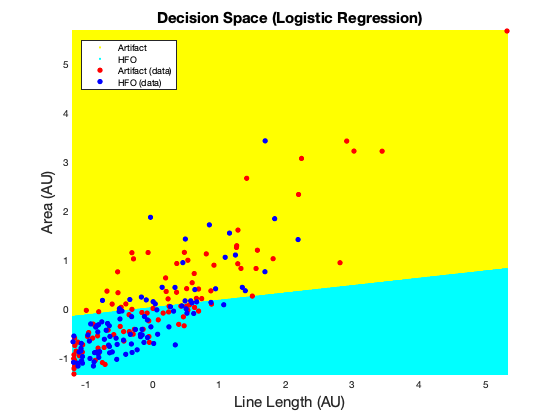
\includegraphics [width=5in]{spatank_hw4_04.png}


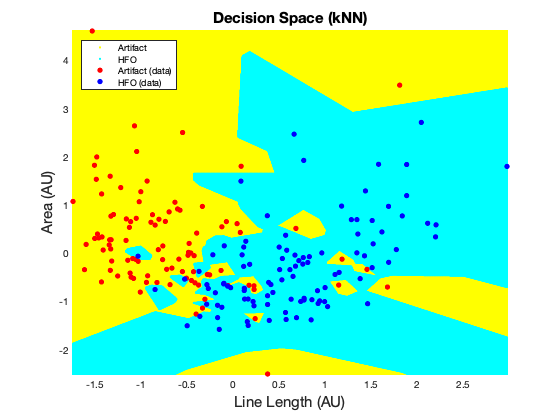
\includegraphics [width=5in]{spatank_hw4_05.png}


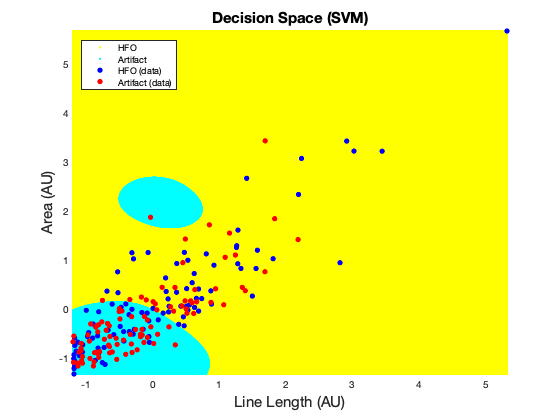
\includegraphics [width=5in]{spatank_hw4_06.png}

 \item In a few sentences, report some observations about the three
 plots, especially similarities and differences between them. Which
 of these has overfit the data the most? Which has underfit the data
 the most? (3 pts)

\begin{lstlisting}
% [ANSWER HERE]
\end{lstlisting}

\end{enumerate}
\section{Cross-Validation (17 pts)} In this section, you will
investigate the importance of cross-validation, which is essential
for choosing the tunable parameters of a model (as opposed to the
internal parameters the the classifier ``learns'' by itself on the
training data).
\begin{enumerate}
 \item Since you cannot do any validation on the testing set, you'll
 have to split up the training set. One way of doing this is to
 randomly split it into $k$ unique ``folds,'' with roughly the same
 number of samples ($n/k$ for $n$ total training samples) in each
 fold, training on $k-1$ of the folds and doing predictions on the
 remaining one.
 In this section, you will do 10-fold cross-validation, so create a
 cell array\footnote{A cell array is slightly different from a
 normal Matlab numeric array in that it can hold elements of
 variable size (and type), for example \texttt{folds\{1\} = [1 3 6]; folds\{2\}
 = [2 5]; folds\{3\} = [4 7];}.} \texttt{folds} that contains 10
 elements, each of which is itself an array of the indices of
 training samples in that fold. You may find the \texttt{randperm}
 function useful for this.
 Using the command \texttt{length(unique([folds\{:\}]))}, show that
 you have 200 unique sample indices (i.e. there are no repeats
 between folds). (2 pts)

\begin{lstlisting}
% [ANSWER HERE]

num_folds = 10; % number of CV folds
rand_idx = randperm(length(trainFeatsNorm));
folds = mat2cell(reshape(rand_idx, num_folds, []), ones(1, 10));

length(unique([folds{:}]))
\end{lstlisting}

\color{lightgray} \begin{lstlisting}
ans =

   200

\end{lstlisting} \color{black}

 \item Train a new $k$-NN model (still using the default parameters)
 on the folds you just created. Predict the labels for each fold
 using a classifier trained on all the other folds. After running
 through all the folds, you will have label predictions for each
 training sample.
  \begin{enumerate}
   \item Compute the error (called the validation error) of these
   predictions. (3 pts)

\begin{lstlisting}
% [ANSWER HERE]

train_errors_CV = zeros(1, num_folds);
val_errors_CV = zeros(1, num_folds);

for i = 1:num_folds
    fold_train_data = trainFeatsNorm;
    fold_train_labels = trainLabels;
    fold_train_data(folds{i, 1}, :) = []; % remove one fold for validation
    fold_train_labels(folds{i, 1}, :) = []; % remove one fold for validation

    fold_val_data = trainFeatsNorm(folds{i, 1}, :);
    fold_val_labels = trainLabels(folds{i, 1}, :);

    Mdl_kNN = fitcknn(fold_train_data, fold_train_labels);

    fold_train_labels_pred = predict(Mdl_kNN, fold_train_data);
    train_errors_CV(i) = sum(fold_train_labels ~= fold_train_labels_pred)/length(fold_train_labels);

    fold_val_labels_pred = predict(Mdl_kNN, fold_val_data);
    val_errors_CV(i) = sum(fold_val_labels ~= fold_val_labels_pred)/length(fold_val_labels);
end

val_error = mean(val_errors_CV)
\end{lstlisting}

\color{lightgray} \begin{lstlisting}
val_error =

    0.5850

\end{lstlisting} \color{black}

\item How does this error compare (lower,
   higher, the same?) to the error you found in question 3.3? Does
   it make sense? (2 pts)

\begin{lstlisting}
% [ANSWER HERE]
\end{lstlisting}

  \end{enumerate}
 \item Create a parameter space for your $k$-NN model by setting a
 vector of possible $k$ values from 1 to 30. For each values of $k$,
 calculate the validation error and average training error over the
 10 folds.
  \begin{enumerate}
   \item Plot the training and validation error values over the
   values of $k$, using the formatting string \texttt{'b-o'} for the
   validation error and \texttt{'r-o'} for the training error. (4
   pts)

\begin{lstlisting}
% [ANSWER HERE]

ks = 1:30;
train_errors_ks = zeros(1, length(ks));
val_errors_ks = zeros(1, length(ks));

for i = 1:length(ks)
    k = ks(i);
    train_errors_CV = zeros(1, num_folds);
    val_errors_CV = zeros(1, num_folds);
    for j = 1:num_folds
        fold_train_data = trainFeatsNorm;
        fold_train_labels = trainLabels;
        fold_train_data(folds{j, 1}, :) = []; % remove one fold for validation
        fold_train_labels(folds{j, 1}, :) = []; % remove one fold for validation

        fold_val_data = trainFeatsNorm(folds{j, 1}, :);
        fold_val_labels = trainLabels(folds{j, 1}, :);

        Mdl_kNN = fitcknn(fold_train_data, fold_train_labels, ...
            'NumNeighbors', k);

        fold_train_labels_pred = predict(Mdl_kNN, fold_train_data);
        train_errors_CV(j) = sum(fold_train_labels ~= ...
            fold_train_labels_pred)/length(fold_train_labels);

        fold_val_labels_pred = predict(Mdl_kNN, fold_val_data);
        val_errors_CV(j) = sum(fold_val_labels ~= ...
            fold_val_labels_pred)/length(fold_val_labels);
    end
    train_errors_ks(i) = mean(train_errors_CV);
    val_errors_ks(i) = mean(val_errors_CV);
end

figure;
hold on
plot(ks, train_errors_ks, 'r-o', 'LineWidth', 2);
plot(ks, val_errors_ks, 'b-o', 'LineWidth', 2);
legend('Training Error', 'Validation Error', 'Location', 'SouthEast');
hold off
xlabel('k', 'FontSize', 15);
ylabel('Error (AU)', 'FontSize', 15);
title('Parameter Selection (k)', 'FontSize', 15);
\end{lstlisting}


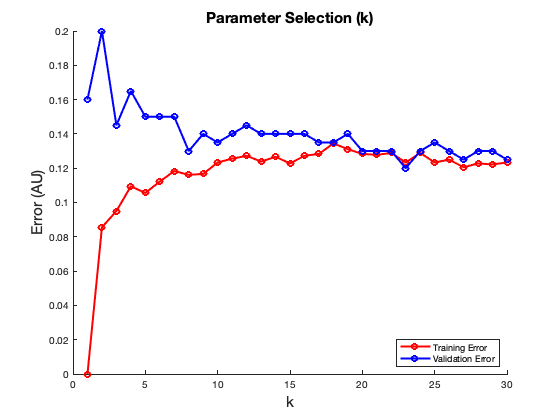
\includegraphics [width=5in]{spatank_hw4_07.png}

\item What is the optimal $k$ value and its training and testing error? (1 pts)

\begin{lstlisting}
% [ANSWER HERE]

[~, k_opt] = min(val_errors_ks);
k_opt_train_error = train_errors_ks(k_opt)
k_opt_val_error = val_errors_ks(k_opt)
\end{lstlisting}

\color{lightgray} \begin{lstlisting}
k_opt_train_error =

    0.2956


k_opt_val_error =

    0.4100

\end{lstlisting} \color{black}

   \item Explain why $k$-NN generally overfits less with higher
   values of $k$. (2 pts)

\begin{lstlisting}
% [ANSWER HERE]

% When $k = 1$, every training point is assigned the label of its
% nearest neighbor, which is itself. This leads to a training error of 0.
% Higher values of $k$ have the effect of distributing the responsibility
% for a point's label amongst multiple training points. This leads to less
% over-fitting.
\end{lstlisting}

  \end{enumerate}
 \item
  \begin{enumerate}
   \item Using your optimal value for $k$ from CV, calculate the
   $k$-NN model's \textit{testing} error. (1 pts)

\begin{lstlisting}
% [ANSWER HERE]

Mdl_kNN_opt = fitcknn(trainFeatsNorm, trainLabels, 'NumNeighbors', k_opt);

trainLabelsPred = predict(Mdl_kNN_opt, trainFeatsNorm);

testLabelsPred = predict(Mdl_kNN_opt, testFeatsNorm);
test_error_knn_k_opt = sum(testLabels ~= testLabelsPred)/length(testLabels)
\end{lstlisting}

\color{lightgray} \begin{lstlisting}
test_error_knn_k_opt =

    0.5476

\end{lstlisting} \color{black}

\item How does this
   model's testing error compare to the $k$-NN model
   you trained in question 3.3? Is it the best of the three models
   you trained in Section 3? (2 pts)

\begin{lstlisting}
% [ANSWER HERE]
\end{lstlisting}

  \end{enumerate}
\end{enumerate}




\end{document}
    
